% Options for packages loaded elsewhere
\PassOptionsToPackage{unicode}{hyperref}
\PassOptionsToPackage{hyphens}{url}
%
\documentclass[
]{book}
\usepackage{lmodern}
\usepackage{amssymb,amsmath}
\usepackage{ifxetex,ifluatex}
\ifnum 0\ifxetex 1\fi\ifluatex 1\fi=0 % if pdftex
  \usepackage[T1]{fontenc}
  \usepackage[utf8]{inputenc}
  \usepackage{textcomp} % provide euro and other symbols
\else % if luatex or xetex
  \usepackage{unicode-math}
  \defaultfontfeatures{Scale=MatchLowercase}
  \defaultfontfeatures[\rmfamily]{Ligatures=TeX,Scale=1}
  \setmainfont[]{Arial}
  \setmathfont[]{Fira Math Regular}
\fi
% Use upquote if available, for straight quotes in verbatim environments
\IfFileExists{upquote.sty}{\usepackage{upquote}}{}
\IfFileExists{microtype.sty}{% use microtype if available
  \usepackage[]{microtype}
  \UseMicrotypeSet[protrusion]{basicmath} % disable protrusion for tt fonts
}{}
\makeatletter
\@ifundefined{KOMAClassName}{% if non-KOMA class
  \IfFileExists{parskip.sty}{%
    \usepackage{parskip}
  }{% else
    \setlength{\parindent}{0pt}
    \setlength{\parskip}{6pt plus 2pt minus 1pt}}
}{% if KOMA class
  \KOMAoptions{parskip=half}}
\makeatother
\usepackage{xcolor}
\IfFileExists{xurl.sty}{\usepackage{xurl}}{} % add URL line breaks if available
\IfFileExists{bookmark.sty}{\usepackage{bookmark}}{\usepackage{hyperref}}
\hypersetup{
  pdftitle={Evan's PhD thesis proposal},
  pdfauthor={Evan C Mascitti},
  hidelinks,
  pdfcreator={LaTeX via pandoc}}
\urlstyle{same} % disable monospaced font for URLs
\usepackage{longtable,booktabs}
% Correct order of tables after \paragraph or \subparagraph
\usepackage{etoolbox}
\makeatletter
\patchcmd\longtable{\par}{\if@noskipsec\mbox{}\fi\par}{}{}
\makeatother
% Allow footnotes in longtable head/foot
\IfFileExists{footnotehyper.sty}{\usepackage{footnotehyper}}{\usepackage{footnote}}
\makesavenoteenv{longtable}
\usepackage{graphicx}
\makeatletter
\def\maxwidth{\ifdim\Gin@nat@width>\linewidth\linewidth\else\Gin@nat@width\fi}
\def\maxheight{\ifdim\Gin@nat@height>\textheight\textheight\else\Gin@nat@height\fi}
\makeatother
% Scale images if necessary, so that they will not overflow the page
% margins by default, and it is still possible to overwrite the defaults
% using explicit options in \includegraphics[width, height, ...]{}
\setkeys{Gin}{width=\maxwidth,height=\maxheight,keepaspectratio}
% Set default figure placement to htbp
\makeatletter
\def\fps@figure{htbp}
\makeatother
\setlength{\emergencystretch}{3em} % prevent overfull lines
\providecommand{\tightlist}{%
  \setlength{\itemsep}{0pt}\setlength{\parskip}{0pt}}
\setcounter{secnumdepth}{5}
\usepackage{booktabs}
\ifluatex
  \usepackage{selnolig}  % disable illegal ligatures
\fi
\usepackage[]{natbib}
\bibliographystyle{apalike}

\title{Evan's PhD thesis proposal}
\author{Evan C Mascitti}
\date{last updated 2020-10-23}

\begin{document}
\maketitle

{
\setcounter{tocdepth}{1}
\tableofcontents
}
\hypertarget{introduction}{%
\chapter{Introduction}\label{introduction}}

The production of artificial soils has received much study. However, there are
no published scientific experiments on this topic as it pertains to baseball and
softball fields.

\hypertarget{purpose}{%
\chapter{Purpose}\label{purpose}}

The purpose of my thesis is to create a new way to think about the soils used on baseball and softball infields.

\hypertarget{objectives-and-deliverables}{%
\section{Objectives and deliverables}\label{objectives-and-deliverables}}

The deliverables from this project are:

\begin{enumerate}
\def\labelenumi{\arabic{enumi}.}
\tightlist
\item
  a general framework for understanding the behavior of sand-clay mixes in a quantitative way
\item
  specific recommendations for the ratios which common clayey soils should be mixed with sand for optimal performance at any maintenance level
\item
  suggestions for how to beneficiate poorly-performing clay soils with other kinds of clays to maximize the locally available materials by ``spiking'' the local clay with a small percentage of imported solum
\end{enumerate}

\hypertarget{review-of-literature}{%
\chapter{Review of literature}\label{review-of-literature}}

\hypertarget{soil-mixtures-for-baseball-and-softball-infields}{%
\section{Soil mixtures for baseball and softball infields}\label{soil-mixtures-for-baseball-and-softball-infields}}

Baseball was first played in the early 19th century, but the definitive origins of the game are likely lost to history \citep{Walker1994}. The earliest recorded attempt to alter the physical properties of an infield soil were by Harry Wright in 1875. Wright and his contemporaries incorporated various materials into their infield soils to enhance stability, firmness, or drainage of the playing surface. Amendments included organic debris (straw, ashes) and and inorganic materials (sand, lime, cinders) \citep{Morris2007}.

Infield soil mixes were produced off-site and imported beginning in the 1960s ?Zwasksa?.

\citet{Goodall2005} is the only published account of research on infield soil mixtures. The authors installed several soils which were commercially available within their region.

\citet{Brosnan2008a} surveyed the surface conditions of the infield skin on extant playing fields at three maintenance levels. Particle size analyses were performed on soil sampled from each infield skin. The USDA soil texture of those samples is plotted in \ref{fig:brosnan-survey-usda}. These soils were sampled from the upper 13 mm and contained large granules of calcined clay infield conditioner; therefore, the texture measured with this method is coarser than the ``true'' texture of the base soil.

\begin{figure}

{\centering 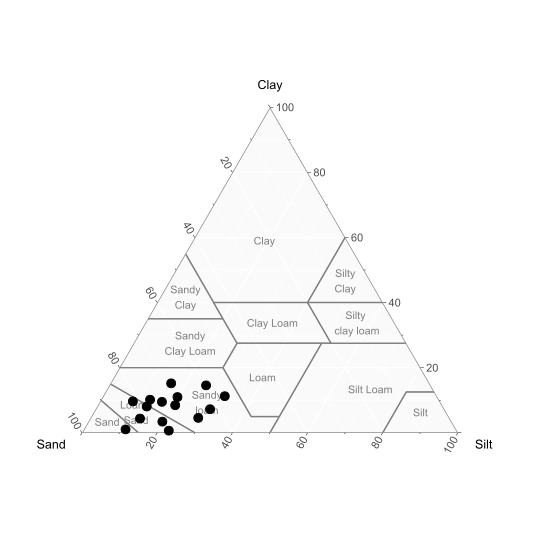
\includegraphics[width=7.5in]{figs/brosnan_survey_PSA} 

}

\caption{Infield soils suyveyed by Brosnan (2008a)}\label{fig:brosnan-survey-usda}
\end{figure}

Additionally, Brosnan et al.~published research on the infield skin's role in athlete-to-surface interactions \citeyearpar{Brosnan2009} and ball-to-surface interactions \citeyearpar{Brosnan2011}. Bulk density (\(\Large{\rho}\small{_{bulk}}\)) was shown to influence surface properties, although the range of bulk densities tested (1.2 - 1.8 Mg m\textsuperscript{-3}) was beneath values typically encountered on infield skins (author's personal observation; data not shown).

However, the work of Brosnan et al. \citetext{\citeyear{Brosnan2009}; \citeyear{Brosnan2011}} was performed on a single soil material and focused on construction and maintenance practices rather than mix design.

\hypertarget{laboratory-methods-for-evaluating-soil-behavior-and-physical-properties}{%
\section{Laboratory methods for evaluating soil behavior and physical properties}\label{laboratory-methods-for-evaluating-soil-behavior-and-physical-properties}}

Many soil tests have been developed with the goal of supplanting the Atterberg limits. However, due to the success and the abundance of data which has accumulated using these test methods, they are unlikely to be abandoned.

\hypertarget{definitions-of-soil-behavior-and-physical-properties}{%
\section{Definitions of soil behavior and physical properties}\label{definitions-of-soil-behavior-and-physical-properties}}

Toughness is really the most defining feature of clay soil.

\hypertarget{particle-size-analysis}{%
\subsection{Particle size analysis}\label{particle-size-analysis}}

\hypertarget{compaction-tests}{%
\subsection{Compaction tests}\label{compaction-tests}}

\hypertarget{compression-and-shear-strength-tests}{%
\subsection{Compression and shear strength tests}\label{compression-and-shear-strength-tests}}

\hypertarget{atterberg-limits}{%
\subsection{Atterberg limits}\label{atterberg-limits}}

\hypertarget{toughness-tests}{%
\subsection{Toughness tests}\label{toughness-tests}}

\hypertarget{behavior-of-sand-clay-mixtures}{%
\section{Behavior of sand-clay mixtures}\label{behavior-of-sand-clay-mixtures}}

The Atterberg limits and unconfined compression testing are the primary means which have been used to charazcterize soil mixtures. These mixtures may contain two components(sand and clay), or three components (sand and two separate types of clay soil)

\hypertarget{proposed-experiments}{%
\chapter{Proposed experiments}\label{proposed-experiments}}

\hypertarget{chapter-1-a-novel-method-for-measuring-the-performance-of-baseball-and-softball-infield-skin-soils}{%
\section{Chapter 1: A novel method for measuring the performance of baseball and softball infield skin soils}\label{chapter-1-a-novel-method-for-measuring-the-performance-of-baseball-and-softball-infield-skin-soils}}

\hypertarget{chapter-2-toughness-of-clay-soil-near-the-plastic-limit-using-unconfined-compression-tests}{%
\section{Chapter 2: Toughness of clay soil near the plastic limit using unconfined compression tests}\label{chapter-2-toughness-of-clay-soil-near-the-plastic-limit-using-unconfined-compression-tests}}

\hypertarget{chapter-3-a-critical-appraisal-of-particle-size-analysis-as-a-proxy-for-soil-behavior}{%
\section{Chapter 3: A critical appraisal of particle size analysis as a proxy for soil behavior}\label{chapter-3-a-critical-appraisal-of-particle-size-analysis-as-a-proxy-for-soil-behavior}}

\hypertarget{chapter-4-a-rational-theory-of-mix-design-for-blended-soils-used-on-baseball-and-softball-infields}{%
\section{Chapter 4: A rational theory of mix design for blended soils used on baseball and softball infields}\label{chapter-4-a-rational-theory-of-mix-design-for-blended-soils-used-on-baseball-and-softball-infields}}

\hypertarget{references}{%
\chapter{References}\label{references}}

  \bibliography{book.bib,packages.bib,library.bib}

\end{document}
